\typeout{IJCAI-11 Instructions for Authors Modified for Masgist{\`e}re Students}

% These are the instructions for authors for IJCAI-11.
% They are the same as the ones for IJCAI-07 with superficical wording
%   changes only.

\documentclass{article}
% The file ijcai11.sty is the style file for IJCAI-11 (same as ijcai07.sty).
% Use the postscript times font!
\usepackage{ijcai11}
\usepackage{times}%
\usepackage{color, colortbl}
\let\proof\relax
\let\endproof\relax
\usepackage{amsmath,amssymb,amsthm}
\usepackage[utf8]{inputenc}
\usepackage[english]{babel}
\usepackage{graphicx} 
\usepackage{url}
\usepackage{caption}
\usepackage{subcaption}
\usepackage{mathpazo}
\usepackage{booktabs}
\usepackage{hyperref}
\usepackage{tikz}
\usepackage[]{algorithm2e}
\usepackage{subfiles}
\usepackage{esvect}
\usepackage{comment}
\usepackage{upgreek}
\usepackage[
  style=numeric,
  natbib=true,
  sortcites=true,
  block=space]{biblatex}
\bibliography{parts/biblio}%
\DeclareMathOperator*{\argmax}{arg\,max}
\DeclareMathOperator*{\argmin}{arg\,min}
\providecommand{\keywords}[1]{\textbf{\textit{Keywords}} #1}

\begin{document}
\subfile{parts/title.tex}
\maketitle
\subfile{parts/abstract}
\subfile{parts/intro}
\subfile{parts/related}
\subfile{parts/proposed}
\subfile{parts/experiment}
\subfile{parts/conclusion}
\subfile{parts/futur}
\begin{table}
\caption{\label{tab:res_mask}Clustering results for $K$-Means applies to 
different learned latent space to measure the efficiency of lexical constraints
for $K$-Means algorithm. Performance is measured in terms of NMI, Adjusted Rand 
Index and clustering Accuracy, higher is better. Each cell contains the average
and the standard deviation computed over 10 runs.}
%The best result for each  metric/dataset is bold.}
\centering
\resizebox{\hsize}{!}{
\begin{tabular}{|l|l|l|l|}
    \hline
                      & ACC      &ARI       &NMI       \\ \hline
    $K$-Means         &$48.8\pm6.6$&$18.4\pm6.0$&$29.7\pm5.8$\\ \hline
    AE + KM, SP       &$51.3\pm3.5$&$17.5\pm5.8$&$24.5\pm5.1$\\ \hline
    Deep $K$-Means    &$54.4\pm4.9$&$23.9\pm3.5$&$29.6\pm3.6$\\ \hline
    AE + KM, LP mask  &$65.0\pm6.7$&$35.6\pm7.3$&$37.5\pm6.5$\\ \hline
    AE + KM, LP sim   &$62.7\pm6.1$&$35.1\pm5.7$&$38.4\pm4.1$\\ \hline
       CDKM, LP mask  &\boldmath$72.7\pm4.0$&\boldmath$43.8\pm5.4$&\boldmath$44.1\pm3.9$\\ \hline
       CDKM, LP sim   &$72.5\pm4.5$&$43.7\pm5.7$&$44.0\pm4.3$\\ \hline
       CDKM, SP mask  &$70.3\pm4.2$&$41.0\pm5.1$&$42.1\pm4.0$\\ \hline
       CDKM, SP sim   &$70.4\pm5.1$&$41.8\pm7.1$&$43.0\pm5.2$\\ \hline
       
\end{tabular}
}
\subcaption*{RCV1}
\resizebox{\hsize}{!}{
\begin{tabular}{|l|l|l|l|}
    \hline
                      & ACC      &ARI       &NMI       \\ \hline
    $K$-Means         &$36.1\pm2.2$&$13.3\pm1.7$&$40.9\pm1.6$\\ \hline
    AE + KM, SP       &$53.1\pm2.3$&$35.0\pm1.4$&$49.3\pm1.0$\\ \hline
    Deep $K$-Means    &$54.9\pm1.7$&$37.6\pm1.1$&$51.6\pm0.6$\\ \hline
    AE + KM, LP mask  &$56.8\pm1.7$&$38.4\pm1.1$&$51.6\pm0.6$\\ \hline
    AE + KM, LP sim   &$56.0\pm2.3$&$37.6\pm1.6$&$50.8\pm0.7$\\ \hline
       CDKM, LP mask  &\boldmath$61.3\pm0.6$&\boldmath$41.2\pm0.8$&$52.7\pm0.5$\\ \hline
       CDKM, LP sim   &$60.6\pm1.3$&$40.5\pm1.3$&$53.0\pm0.8$\\ \hline
       CDKM, SP mask  &$60.2\pm1.8$&\boldmath$41.2\pm0.9$&\boldmath$53.5\pm0.5$\\ \hline
       CDKM, SP sim   &$60.5\pm1.2$&$40.7\pm0.8$&$52.9\pm0.5$\\ \hline
\end{tabular}
}
\subcaption*{20 Newsgroups}
\resizebox{\hsize}{!}{
\begin{tabular}{|l|l|l|l|}
    \hline
                      & ACC      &ARI       &NMI       \\ \hline
    $K$-Means         &$33.1\pm2.7$&$ 8.7\pm1.3$&$26.3\pm1.6$\\ \hline
    AE + KM, SP       &$45.2\pm3.3$&$23.0\pm2.5$&$30.0\pm2.0$\\ \hline
    Deep $K$-Means    &$44.5\pm2.4$&$23.6\pm2.4$&$30.2\pm2.0$\\ \hline
    AE + KM, LP mask  &$45.9\pm2.2$&$24.0\pm1.8$&$31.8\pm1.5$\\ \hline
    AE + KM, LP sim   &$46.2\pm2.6$&$24.6\pm1.9$&$32.3\pm1.3$\\ \hline
       CDKM, LP mask  &$50.0\pm2.1$&$26.0\pm1.6$&$31.7\pm1.7$\\ \hline
       CDKM, LP sim   &$49.4\pm2.1$&$25.3\pm1.9$&$31.1\pm1.7$\\ \hline
       CDKM, SP mask  &$49.5\pm1.7$&$26.1\pm1.1$&$32.0\pm0.9$\\ \hline
       CDKM, SP sim   &$49.3\pm1.1$&$25.9\pm1.2$&$32.0\pm1.1$\\ \hline
\end{tabular}
}
\subcaption*{20 Newsgroups with noise}
%\resizebox{\hsize}{!}{
%\begin{tabular}{|l|l|l|l|}
%    \hline
%                      & ACC        &ARI         &NMI       \\ \hline
%    $K$-Means         &$54.6\pm3.2$&$31.2\pm2.7$&$63.4\pm0.9$\\ \hline
%    AE + KM, SP       &$72.9\pm2.5$&$62.7\pm2.5$&$72.8\pm1.5$\\ \hline
%    Deep $K$-Means    &$73.6\pm4.8$&$63.5\pm2.9$&$74.6\pm1.3$\\ \hline
%    AE + KM, LP mask  &$00.0\pm0.0$&$00.0\pm0.0$&$00.0\pm0.0$\\ \hline
%    AE + KM, LP sim   &$00.0\pm0.0$&$00.0\pm0.0$&$00.0\pm0.0$\\ \hline
%  CDKM, LP mask  &$00.0\pm0.0$&$00.0\pm0.0$&$00.0\pm0.0$\\ \hline
%       CDKM, LP sim   &$00.0\pm0.0$&$00.0\pm0.0$&$00.0\pm0.0$\\ \hline
%       CDKM, SP mask  &$00.0\pm0.0$&$00.0\pm0.0$&$00.0\pm0.0$\\ \hline
%       CDKM, SP sim   &$00.0\pm0.0$&$00.0\pm0.0$&$00.0\pm0.0$\\ \hline
%\end{tabular}
%}
%\subcaption*{DBPedia}
\end{table}

\begin{table}
\caption{\label{tab:res_non_discr}Clustering results for $K$-Means applies applies to 
different learned latent space to measure the efficiency of lexical constraints
for $K$-Means algorithm. Performance is measured in terms of NMI, Adjusted Rand 
Index and clustering Accuracy, higher is better. Each cell contains the average
and the standard deviation computed over 10 runs.}
%The best result for each  metric/dataset is bold.}
\centering
\resizebox{\hsize}{!}{
\begin{tabular}{|l|l|l|l|}
    \hline
                      & ACC      &ARI       &NMI       \\ \hline
    $K$-Means         &$48.8\pm6.6$&$18.4\pm6.0$&$29.7\pm5.8$\\ \hline
    AE + KM, SP       &$51.3\pm3.5$&$17.5\pm5.8$&$24.5\pm5.1$\\ \hline
    Deep $K$-Means    &$54.4\pm4.9$&$23.9\pm3.5$&$29.6\pm3.6$\\ \hline
    AE + KM, LP mask  &$66.1\pm5.0$&$38.2\pm5.3$&$40.5\pm4.3$\\ \hline
    AE + KM, LP sim   &$62.3\pm4.8$&$35.2\pm5.0$&$38.7\pm3.5$\\ \hline
       CDKM, LP mask  &\boldmath$68.5\pm5.6$&\boldmath$39.6\pm6.4$&\boldmath$41.3\pm4.6$\\ \hline
       CDKM, LP sim   &$65.8\pm5.0$&$36.2\pm5.5$&$38.9\pm3.7$\\ \hline
       CDKM, SP mask  &$68.5\pm5.6$&$39.6\pm6.4$&$41.3\pm4.6$\\ \hline
       CDKM, SP sim   &$67.5\pm6.3$&$38.6\pm6.4$&$40.7\pm4.4$\\ \hline
\end{tabular}
}
\subcaption*{RCV1}
\resizebox{\hsize}{!}{
\begin{tabular}{|l|l|l|l|}
    \hline
                      & ACC      &ARI       &NMI       \\ \hline
    $K$-Means         &$36.1\pm2.2$&$13.3\pm1.7$&$40.9\pm1.6$\\ \hline
    AE + KM, SP       &$53.1\pm2.3$&$35.0\pm1.4$&$49.3\pm1.0$\\ \hline
    Deep $K$-Means    &$54.9\pm1.7$&$37.6\pm1.1$&$51.6\pm0.6$\\ \hline
    AE + KM, LP mask  &$57.5\pm2.8$&$39.6\pm1.7$&$51.6\pm1.4$\\ \hline
    AE + KM, LP sim   &$55.7\pm1.7$&$37.6\pm1.0$&$50.8\pm0.4$\\ \hline
       CDKM, LP mask  &$58.8\pm1.4$&$38.5\pm1.4$&$52.6\pm0.6$\\ \hline
       CDKM, LP sim   &\boldmath$60.1\pm2.1$&\boldmath$40.2\pm1.4$&\boldmath$52.8\pm1.0$\\ \hline
       CDKM, SP mask  &$58.9\pm2.0$&$38.9\pm1.6$&\boldmath$52.8\pm0.9$\\ \hline
       CDKM, SP sim   &$60.1\pm1.7$&$40.1\pm1.5$&$52.7\pm0.7$\\ \hline
\end{tabular}
}
\subcaption*{20 Newsgroups}
\resizebox{\hsize}{!}{
\begin{tabular}{|l|l|l|l|}
    \hline
                      & ACC      &ARI       &NMI       \\ \hline
    $K$-Means         &$33.1\pm2.7$&$ 8.7\pm1.3$&$26.3\pm1.6$\\ \hline
    AE + KM, SP       &$45.2\pm3.3$&$23.0\pm2.5$&$30.0\pm2.0$\\ \hline
    Deep $K$-Means    &$44.5\pm2.4$&$23.6\pm2.4$&$30.2\pm2.0$\\ \hline
    AE + KM, LP mask  &$45.2\pm2.2$&$24.2\pm1.6$&$32.4\pm1.1$\\ \hline
    AE + KM, LP sim   &$42.3\pm2.4$&$21.7\pm2.0$&$29.1\pm1.3$\\ \hline
       CDKM, LP mask   &$48.8\pm2.3$&\boldmath$25.7\pm1.9$&\boldmath$31.6\pm1.9$\\ \hline
       CDKM, LP sim  &$47.8\pm2.6$&$24.3\pm1.8$&$30.8\pm1.7$\\ \hline
       CDKM, SP mask  &$48.8\pm2.3$&$25.7\pm1.9$&$31.6\pm1.9$\\ \hline
       CDKM, SP sim   &\boldmath$49.2\pm2.3$&$25.2\pm2.0$&$31.5\pm1.7$\\ \hline
\end{tabular}
}
\subcaption*{20 Newsgroups with noise}
%\resizebox{\hsize}{!}{
%\begin{tabular}{|l|l|l|l|}
%    \hline
%                      & ACC        &ARI         &NMI       \\ \hline
%    $K$-Means         &$54.6\pm3.2$&$31.2\pm2.7$&$63.4\pm0.9$\\ \hline
%    AE + KM, SP       &$72.9\pm2.5$&$62.7\pm2.5$&$72.8\pm1.5$\\ \hline
%    Deep $K$-Means    &$73.6\pm4.8$&$63.5\pm2.9$&$74.6\pm1.3$\\ \hline
%    AE + KM, LP mask  &$00.0\pm0.0$&$00.0\pm0.0$&$00.0\pm0.0$\\ \hline
%    AE + KM, LP sim   &$00.0\pm0.0$&$00.0\pm0.0$&$00.0\pm0.0$\\ \hline
%  CDKM, LP mask  &$00.0\pm0.0$&$00.0\pm0.0$&$00.0\pm0.0$\\ \hline
%       CDKM, LP sim   &$00.0\pm0.0$&$00.0\pm0.0$&$00.0\pm0.0$\\ \hline
%       CDKM, SP mask  &$00.0\pm0.0$&$00.0\pm0.0$&$00.0\pm0.0$\\ \hline
%       CDKM, SP sim   &$00.0\pm0.0$&$00.0\pm0.0$&$00.0\pm0.0$\\ \hline
%\end{tabular}
%}
%\subcaption*{DBPedia}
\end{table}

\begin{figure}
  \begin{subfigure}[b]{\hsize}
    \centering
    \fbox{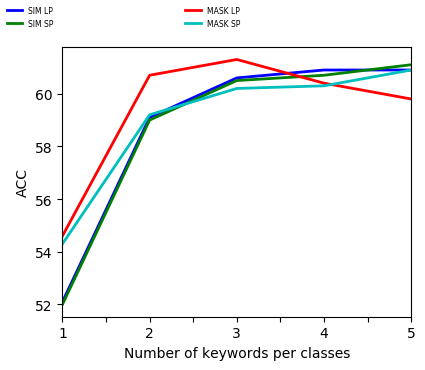
\includegraphics[scale=0.82]{parts/res/dat_file/acc/20NEWS_ACC.png}}     
  \end{subfigure}
  \begin{subfigure}[b]{\hsize}
    \centering
    \fbox{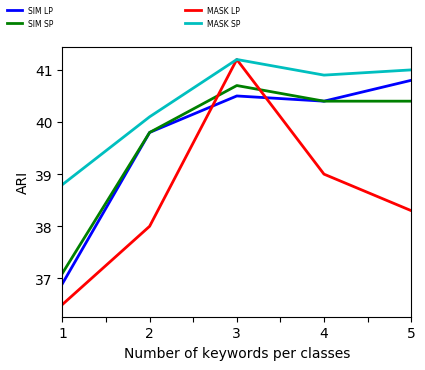
\includegraphics[scale=0.82]{parts/res/dat_file/ari/20NEWS_ARI.png}}    
  \end{subfigure}
  \begin{subfigure}[b]{\hsize}
    \centering
    \fbox{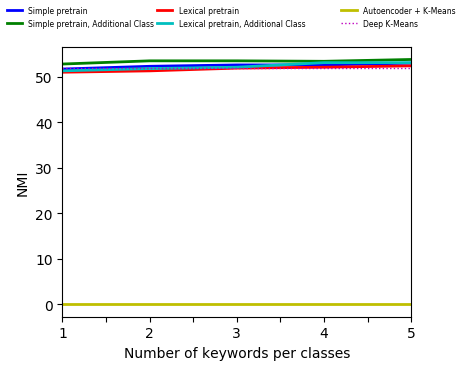
\includegraphics[scale=0.82]{parts/res/dat_file/nmi/20NEWS_NMI.png}}    
  \end{subfigure}\caption{\label{fig:20news}Results for 20 newsgroups dataset}
\end{figure}

\nocite{*}
\newpage
\printbibliography[title=References]
\end{document}
% end of file template.tex
